\section{系统开发与实现}

\subsection{自顶而下开发}

自顶向下设计模式是一种逐步求精、由粗略定性到细节定义的程序的设计过程和设计方法。对要完成的任务进行逐层分解,先对最高层次中的系统需求进行定义、设计、编程以及测试,而将其中未解决的问题选择保留下来,并作为放至下一层次中的一个子任务去解决。按照这样的法则逐层逐个地进行定义、设计、开发和测试,直到所有层次上的问题均能使用目标程序来解决,就能设计出具有一定层次结构的应用程序或应用系统。

所以,首先要求开发者必须对所设计的系统有一个全面的理解。然后才能从顶层开始连续逐层地向下分解,最终分解到所有模块都能用具体的程序逻辑运行,这就能具有逻辑地构造整个程序系统。

在答辩系统开发过程中,采用了自顶而下的设计,并且在顶层设计时将 UI 设计完成,这相比于很多初学者在编写业务逻辑代码的同时,顺便实现的 UI 相比,由于在设计阶段已经完成了页面的设计,最终拥有了更美观的展示效果。这给开发者带来的问题在于:我们应该让设计驱动产品,还是让技术驱动产品。对于大多数情况而言,由设计驱动的产品才是更能够被用户接受的产品。

应用程序开发中的面向用户设计包括用户界面设计(UI)和用户体验设计(UE)。其中,用户体验需要贯穿在一切项目设计和思维创新的过程中。随着计算机技术以及互联网技术的迅速发展,用户体验得到了更多的重视,IT 应用领域内,用户体验设计逐渐在软件设计、互联网设计中占据主要位置。而在信息技术支撑下的创新模式,也是作为面向未来的创新 2.0 模式,在更加广阔的领域强调以人为本、关注用户使用体验。

\subsection{基于 Git 的团队协作}

Git 是一个版本控制系统,用于跟踪计算机文件的变化,并在多个人员之间协调对这些文件的工作。它主要用于软件开发中的源代码版本控制,同时它也可以用来跟踪我们的任何一个文件的变化过程。作为一个分布式的版本控制系统,它的主要特性是高速、数据完整性和对分布式、非线性工作流的支持。

Git 是由 Linus Torvalds 在 2005 年创建的,当时用于开发 Linux 内核,其他内核开发人员也为其最初的开发做出了贡献。Junio Hamano则是目前的维护者。Git 不同与大多数客户机 — 服务器系统(C/S System),每个计算机上的每个 Git 目录都是一个完整的存储库,具有完整的历史和完整的版本跟踪功能,独立于网络访问或中央服务器。

如图 \ref{git-flow} 所示,Git 的最大优点之一是它的分支功能。与其他集中式的版本控制系统的不同点在于,Git 分支是廉价且易于合并的。这使得特性分支工作流受到许多 Git 用户的欢迎。
特性分支为代码库的每个更改提供一个隔离的环境。当一个开发人员想要开始做一些事情 —— 不管他们有多大或多么小的时候 —— 他们会创建一个新的分支。这确保了主分支总是包含生产质量代码。

\begin{figure}
	\centering
	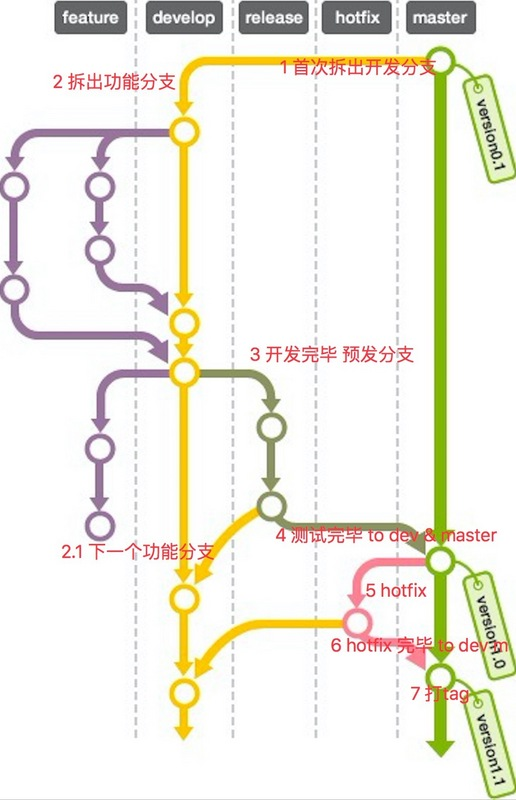
\includegraphics[width=0.6\linewidth]{figure/git-flow}
	\caption{基于 Git 的工作流}
	\label{git-flow}
\end{figure}

使用特性分支不仅比直接编辑生产代码更可靠,而且还提供了有组织的开发。例如,我们答辩系统的每一个特性都在其自己的特性分支中开发并完成处理。

特性分支、分布式开发、Pull Request 和稳定的社区环境的最终结果是一个更快的发布周期。这些功能促进了敏捷的工作流,鼓励开发人员更频繁地共享较小的更改。例如,我们可以配置 Git,以便在任何人将一个 pull 请求合并到测试服务器时,将最新的提交从开发分支部署到测试服务器。将这种构建自动化与单元测试结合,让代码从开发阶段转向生产阶段时,对代码质量拥有最高的信心。

Git 在用户如何管理更新方面提供了很大的灵活性。当在 Git 中与团队合作开发时,确保团队的开发方向是非常重要的。答辩系统在内的对 GMS 系统的二期开发工作由西安石油大学计算机学院 4 名本科学生承担,我们选用了
码云\footnote{码云(Gitee)是在线代码托管平台,由 OSChina 开源中国社区团队基于Git推出,主页:https://gitee.com/}。
提供的 Git 托管服务,而不是诸如 
Github\footnote{GitHub是一个使用Git进行版本控制的基于网络的托管服务,主要用于管理计算机代码。它提供了Git中的所有分布式版本控制功能和大多数源代码的管理功能,以及添加了一些别的特有功能。它为每个项目提供访问控制和多种协作功能,例如错误跟踪、功能请求、任务管理和维基等,主页:https://github.com/} 
这样的国外服务主要原因在于:

\begin{itemize}
	\item 国内的服务拥有更快的访问速度
	\item 私有库功能对个人开发者免费
	\item 线上自动代码质量分析
	\item 中文语言便于团队成员上手
\end{itemize}

Git非常受欢迎,被广泛使用,并被开发人员社区中绝大多数人接受为标准版本控制系统。在大量的Git用户组成的社区可以让我们寻求外部帮助并轻松解决问题。答辩系统业务的开发严重依赖于软件开发流程,Git将彻底改变了我们团队创建和交付工作的方式。包括设计、开发、产品管理、上线运行、客户支持在内的各种流程都可以在我们的开发团队中使用Git轻松处理和维护。


\subsection{对开源项目的有效利用}

开放源代码软件(OSS)是一种计算机软件,其源代码提供许可证,版权持有者有权为任何目的研究,更改和分发软件给任何人。开源软件可能会以公开的协作方式开发。根据研究它的科学家,开源软件是开放式协作的一个突出例子。

对于开发者而言,了解并使用目前在社区中比较流行的开源项目是很必要的一件事。利用这些项目,项目开发工作有时能达到事半功倍的效果。尤其是在互联网这个飞速发展的领域,快速开发、快速上线就是生命,引入开源项目可以节省很多的人力和时间,降低开发成本。Standish Group 2008年的一份报告指出,采用开源软件模式每年可为消费者节省约600亿美元(480亿英镑)的费用。但采用开源软件的决定不应仅仅以低成本为基础。在切换到开源以充分利用它之前,需要对需求进行详细的分析和理解。

包管理器是现在 web 开发必须使用的工具,因为网站系统的开发有必要借助数以万计的众多开源爱好者们的力量。我们的答辩系统由三个包管理器提供支持:Node 自带的 npm,来自Twitter 的 bower 和 Meteor 提供的 Atmosphere  packages。npm 是目前 web 开发最大的包管理平台,我们使用它导入了所需要的 React框架以及相关的包。bower在大多数时候都已被npm代替,但在 Meteor 开发工作流中,由 npm 下载到 /node\_modules 目录下的内容是不能被前端所读取的,并且也不能由我们指定下载到其他目录。所以在该项目开发中,我们使用了bower将一些前端插件下载到了我们指定的/public/bower目录中,这样就可以在浏览器端加载并使用 Chart.js、moment.js 等插件了。

\begin{lstlisting}[title=代码 4-1:答辩系统所选用的全部开源项目列表]
{
	"npm dependencies": {
		"babel-runtime": "^6.26.0",
		"mongodb-backup": "^1.6.9",
		"mongodb-restore": "^1.6.2",
		"react": "^15.6.2",
		"react-addons-pure-render-mixin": "^15.6.2",
		"react-dom": "^15.6.2",
		"react-mixin": "^3.1.1",
		"react-router": "^2.5.2"
	},
	"npm devDependencies": {
		"eslint": "^3.19.0",
		"eslint-plugin-react": "^5.2.2"
	},
	"Bower dependencies": {
		"wangEditor": "2.1.15",
		"jquery": "1.12.4",
		"Chart.js": "chartjs#2.1.6",
		"moment": "2.14.1",
		"PACE": "pace#1.0.2",
		"js-xlsx": "0.8.0",
		"Jdenticon": "jdenticon#1.3.2",
		"docxtemplater": "2.1.5",
		"file-saver": "save-as#1.3.3",
		"jszip-utils": "0.0.2",
		"xlsx-populate": "1.7.0"
	},
	"Atmosphere packages": {
		"meteor-base": "1.0.4",
		"mobile-experience": "1.0.4",
		"mongo": "1.1.14",
		"blaze-html-templates": "1.0.4",
		"reactive-var": "1.0.11",
		"tracker": "1.1.1",
		"standard-minifier-css": "1.3.2",
		"standard-minifier-js": "1.2.1",
		"es5-shim": "4.6.15",
		"ecmascript": "0.5.9",
		"accounts-ui": "1.1.9",
		"accounts-password": "1.3.1",
		"fortawesome:fontawesome": "*",
		"less": "2.7.6",
		"react-meteor-data": "*",
		"jquery": "1.11.10",
		"twbs:bootstrap": "3.3.6",
		"mizzao:bootboxjs": "4.4.0",
		"shell-server": "0.2.1",
		"ostrio:files": "1.9.0"
	}
}
\end{lstlisting}

代码4-1以 JSON 代码的格式列出了答辩系统开发中使用的所有开源项目,可以看到数目相当多,而正是利用了这些方便的开源项目,才使得快速开发一个稳定、强大的业务系统成为可能。

需要注意的是,开源许可软件大多免费提供,但这不一定是这种情况。某些仅允许非商业性质的再分发,或修改源代码仅供个人使用的软件并不属于开源。开放源代码可能有一些限制,特别是关于表达对软件起源的限制,例如要求在代码中保留作者姓名和版权声明,或者要求重新分发许可软件仅在相同的许可证下发布。

本次答辩系统的开发遵循了开源许可协议,其诞生离不开众多开源项目的支持,在此对这些开源项目作者所做出的工作表示感谢。
